% Chapter 3

\chapter{Proposed Methodology} % Write in your own chapter title
\label{Chapter3}
\lhead{Chapter 2. \emph{Proposed Methodology}} % Write in your own chapter title to set the page header

\section{Proposed Solution}
The proposed system focuses on size efficiency of the output video. System acts well in the environment where there is storage issue and bandwidth issue in terms of internet transfer rate. Ultra-durability makes the system more portable to use and more reliable to handle. Re-positionable cameras make the system able to work well in different canvas sizes i.e. size of writing board. System automates the process of video compression technique. Video of the lecture is not recorded as it as video format rather only the important data is extracted. By utilizing the stereo vision and high-speed cameras and low wireless latency, video animation and sound quality is maintained in noisy environment as well. 

\section{General Proposed Model}
General working model of the system can be seen below

\begin{figure}[h]
  \centering
  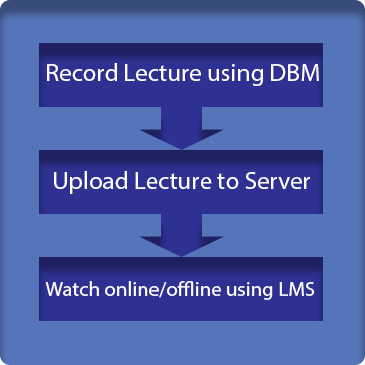
\includegraphics[width=7cm, height=6cm]{General Model}
  \caption{General Methodology View of the System}
\end{figure}


\section{General Flow}
The system consists on several modules and deliverables one of which is controller application. This application is quite important because it include major functionalities and complex image processing algorithms. Furthermore, the instructor in mainly connected to the controller application so that he/she is controlling the recording of lecture i.e. he can start, pause or stop the recording. After the lecture is recorded, he can replay the lecture for any further changes. When the lecture is finally uploaded to central computer, students can play lecture online or save the lecture file in .dbm(file extension) extension to watch later.\\ Offline player is also one of the major modules of the project. It plays the downloaded lecture file just like video player. Learning management system is the online platform where all uploaded online lecture hierarchy is accessible. It is a comprehensive management system designed by placing the convenience of instructor and student in focus. Reliability, security and quality are the top priorities.
A simple visual of the working of system can be seen below
\bigskip
\bigskip

\begin{figure}[h]
  \centering
  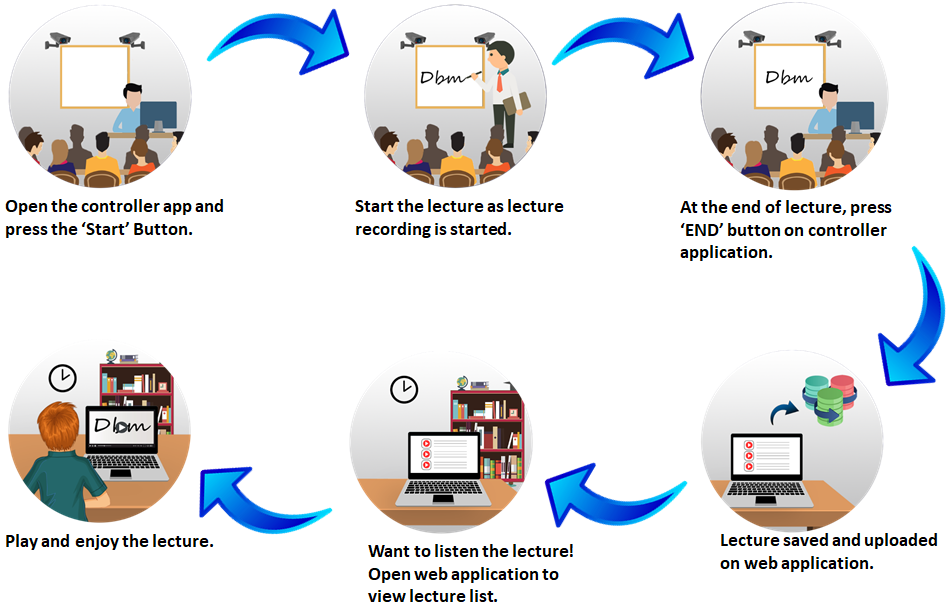
\includegraphics[width=15cm, height=11cm]{Workflow}
  \caption{General Flow of the Project}
\end{figure}
\bigskip

\section{Formulas Used}
\begin{longtable}{|>{\raggedright\arraybackslash}p{3cm}|p{4cm}|p{7cm}|}
\hline
\textbf{Descriptor} & \textbf{Explanation} & \textbf{Formula}\\
\hline
% Row 1 start
\vspace{0pt}\large Euler Angles Rotation Matrices &
Transpose of the fixed-axis matrix. Used in orientation extraction of Board Marker & 
\begin{minipage}{.3\textwidth}
      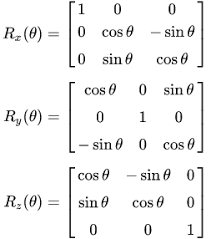
\includegraphics[width=\linewidth, height=60mm, valign=T]{EulerAngles}
\end{minipage}
\\
% Row 1 end
\hline

% Row 1 start
\vspace{0pt}\large Quaternion to Euler conversion &
Used in Marker calibration when an offset is given in particular dimension. & 
\begin{minipage}{.3\textwidth}
      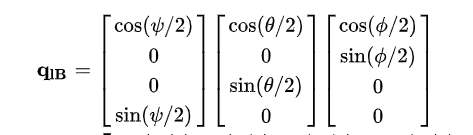
\includegraphics[width=70mm, height=40mm]{Quaternion to Euler conversion}
\end{minipage}
\\
% Row 1 end
\hline



% Row 1 start
\vspace{0pt}\large Euclidean distance formula &
Used to compute the distance in one-dimension. & 
\begin{minipage}{.3\textwidth}
      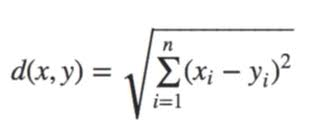
\includegraphics[width=70mm, height=40mm]{Euclidean distance formula}
\end{minipage}
\\
% Row 1 end
\hline


% Row 1 start
\vspace{0pt}\large Equation of line in slope-intercept form &
Used to draw lines and get relative position of Marker with respect to cameras. & 
\bigskip

\begin{minipage}{.3\textwidth}
      
\includegraphics[width=60mm, height=10mm]{slope-intercept form}
\end{minipage}
\\
% Row 1 end
\hline



\caption{Formulae and Equations used}
\end{longtable}

\newpage
\section{Use-Case Diagrams}
To describe the system requirements, use-case diagrams in form of simple user interaction are detailed below
\subsection{Controller Application}
The main end user of controller application is the class instructor or teacher. Teacher use the controller application in
\begin{itemize}

\item Calibrating hardware
\item Record the Lecture
\item Live Stream Lecture
\item Generate Lecture File and annotate it
\item Send Lecture file to Central Server


\end{itemize}

\begin{figure}[h]
  \centering
  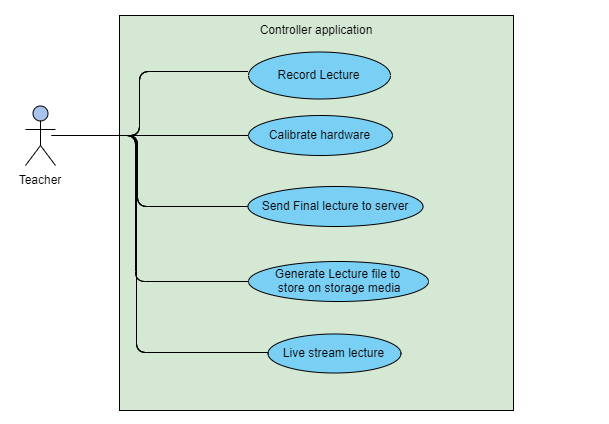
\includegraphics[width=11cm, height=10cm]{ControllerApplication}
  \caption{Use-case Diagram of Controller Application}
\end{figure}

\newpage

\subsection{Player Application}
Just like media player, the player application plays the lecture. Common end user of Player Application is student. Teacher and Student are end users of controller application. Typical actions of Player application are:

\begin{itemize}

\item View Playlist
\item Play Lecture
\item Live Stream Lecture


\end{itemize}

\bigskip

\begin{figure}[h]
  \centering
  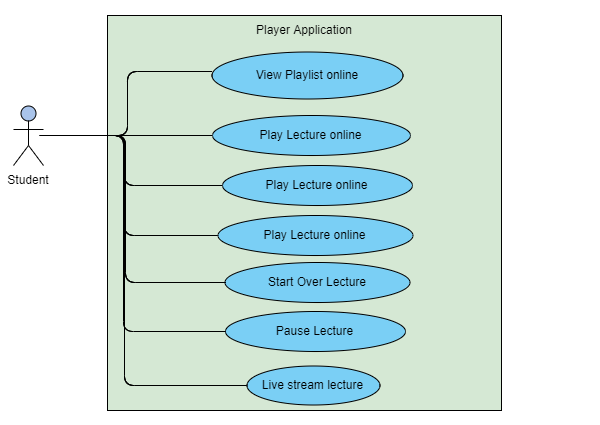
\includegraphics[width=13cm, height=14cm]{PlayerApplication}
  \caption{Use-case Diagram of Player Application}
\end{figure}

\newpage
\subsection{LMS Web Application}
LMS application is major module in terms of accessibility. Students, Teachers and administration can have access to this module simultaneously. LMS functionality is sub-divided into following different users:

\begin{itemize}

\item Admin, who manages the institute.
\item Teacher, who manages students
\item Users, who are students


\end{itemize}

\bigskip

\begin{figure}[h]
  \centering
  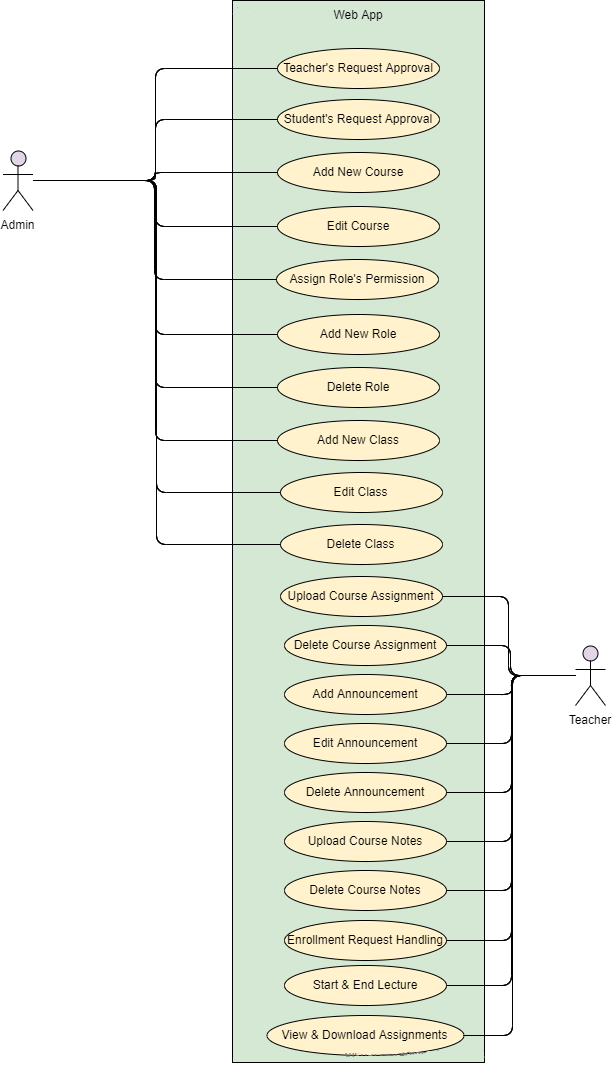
\includegraphics[width=15cm, height=14cm]{DBMUseCaseWebAppPart1}
  \caption{Use-case Diagram of LMS Web Application Part-I}
\end{figure}

\begin{figure}[h]
  \centering
  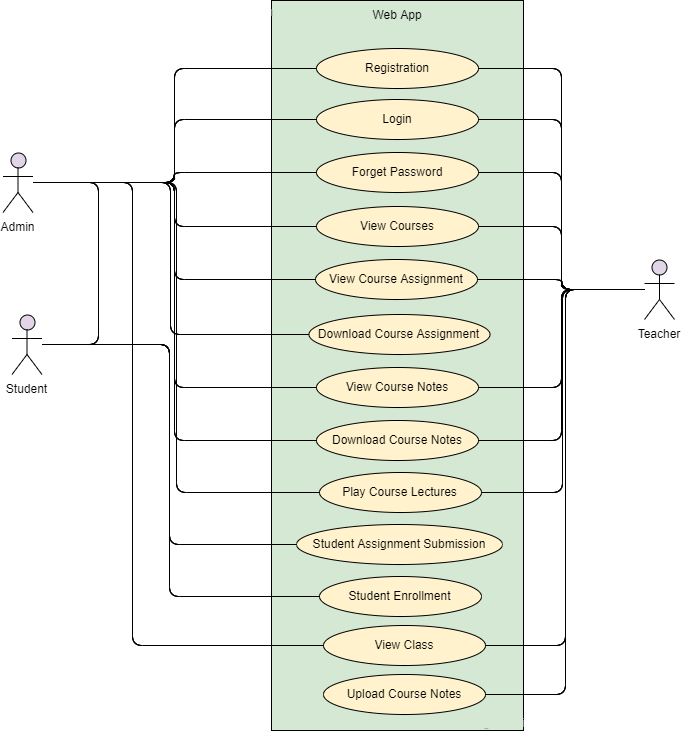
\includegraphics[width=15cm, height=14cm]{DBMUseCaseWebAppPart2}
  \caption{Use-case Diagram of LMS Web Application Part-II}
\end{figure}

\bigskip
\bigskip
\section{Architecture Diagram}
Interaction among different modules of the system is not simple but can be simplified and easy to understand. The set of rules and concepts concerned by the overall project are visually explained by the Architecture Diagram shown below.
It consist of follow modules:
\begin{itemize}

\item Stereo Vision Cameras
\item Marker Hardware
\item Audio Hardware
\item Controller Application
\item Player Application
\item Learning Management System

\end{itemize}
\bigskip
\bigskip

\begin{figure}[h]
  \centering
  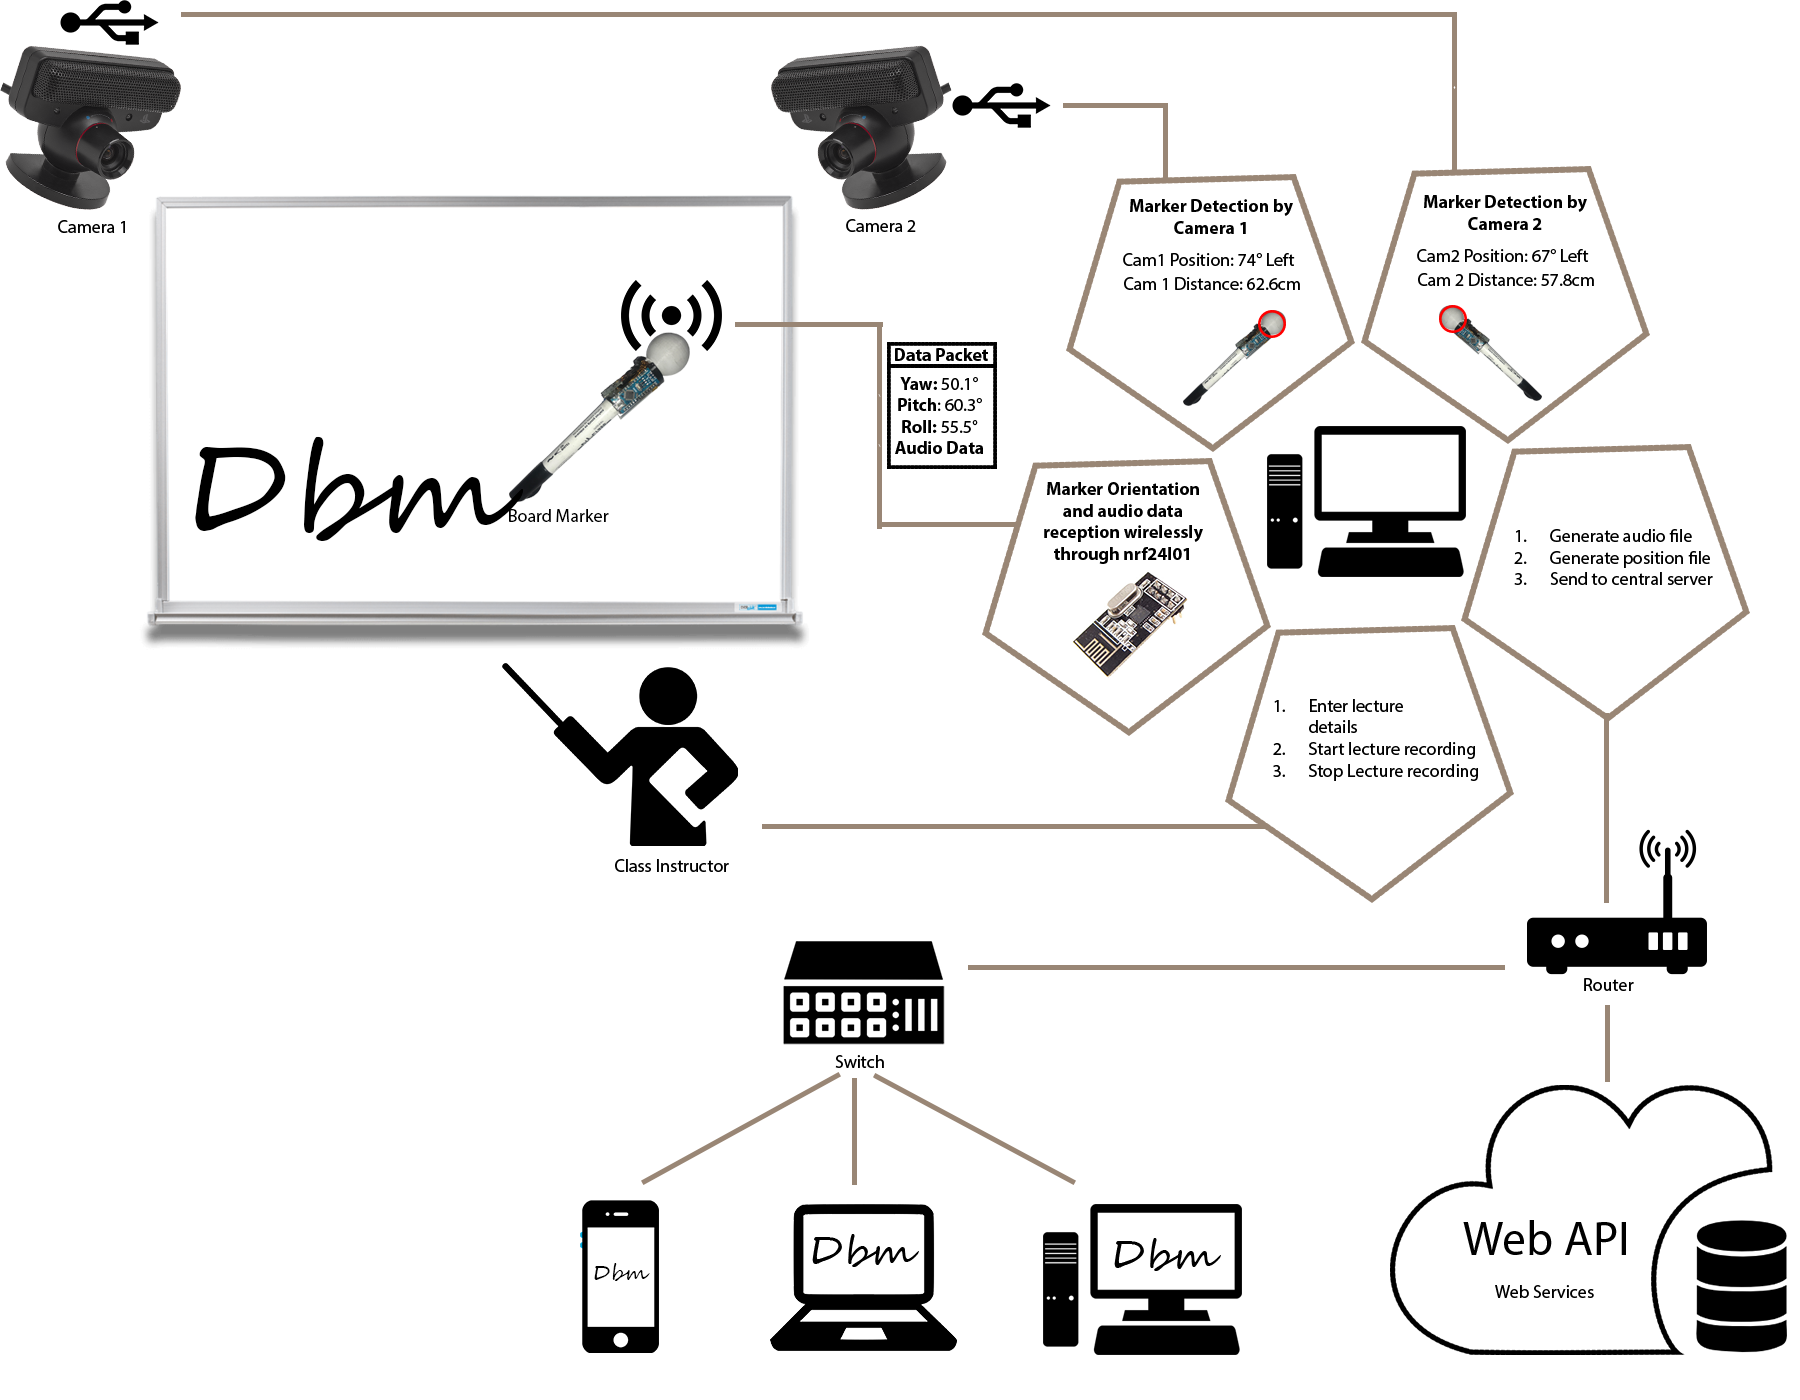
\includegraphics[width=16cm, height=14cm]{Architect 3}
  \caption{Architecture Diagram of Digital Board Marker}
\end{figure}
\bigskip

\section{Modules Methodology Description}
System consists of five major modules. General work flow of each module is detailed using visuals and diagrams.
\subsection{Board Marker}
Board marker transfer the position data of currently written word on the platform i.e. Whiteboard. It is subdivided in two sub-modules
\subsubsection{Stereo Vision Cameras}
At least two high framerate cameras get the video of back ball and send it to controller application. Stereo vision is important for accurately extracting marker position by placing these cameras at such position so that different angles make same alignment to the writing platform irrespective to size. Square and rectangular boards can be mapped to same parent algorithm with simple to calibrate camera placement guide.

\bigskip

\begin{figure}[h]
  \centering
  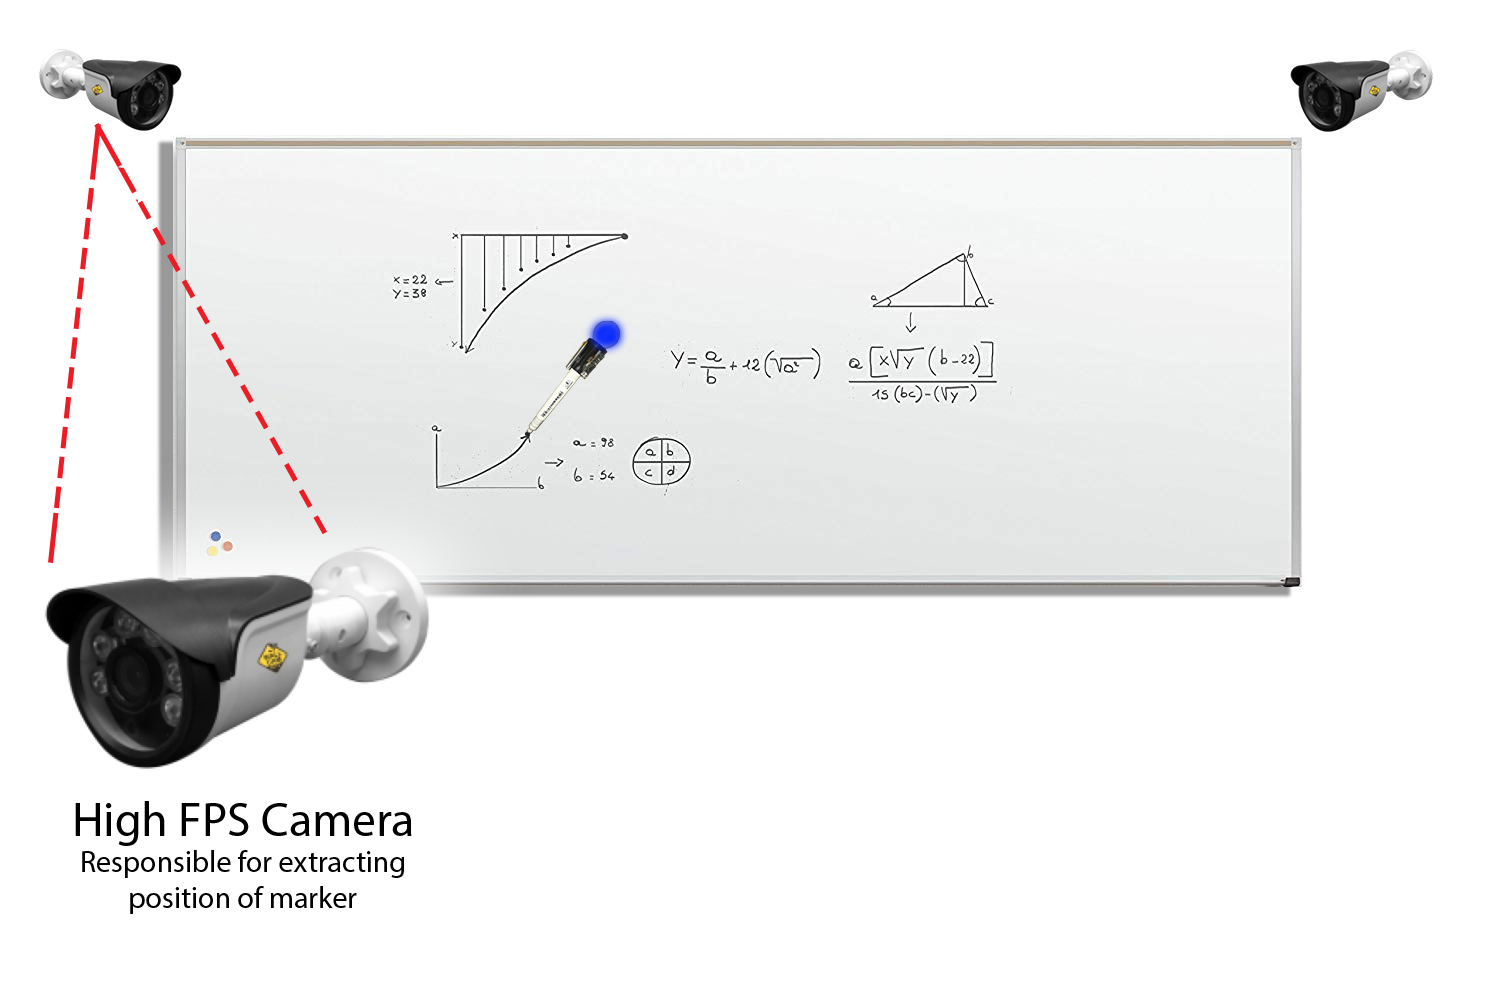
\includegraphics[width=13cm, height=12cm]{Main_Camera}
  \caption{High frame rate camera placement}
\end{figure}

\subsubsection{Marker Hardware}
To extract marker orientation, Marker Hardware is connected to controller application.
\newpage
\bigskip
\bigskip
\begin{figure}[h]
  \centering
  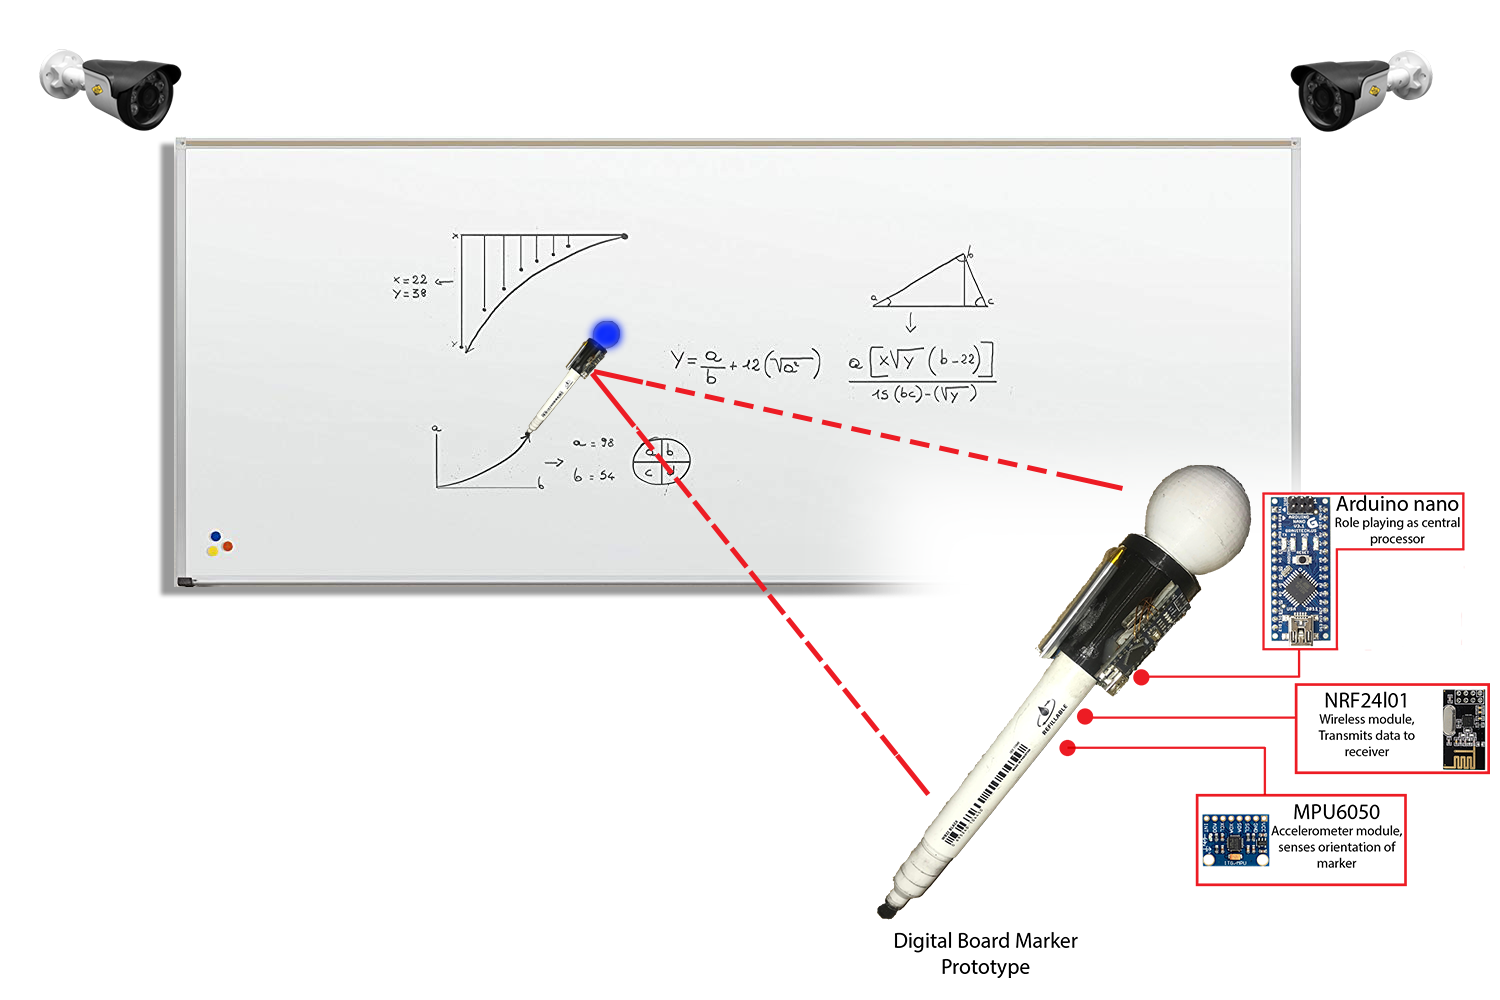
\includegraphics[width=13cm, height=12cm]{Main_Marker}
  \caption{Marker Hardware working methodology}
\end{figure}

\bigskip
\bigskip
\subsection{Audio Hardware}
Wireless voice transmission is done by this module. Voice data is accepted at transmitter module. This data is converted into digital audio. Digital audio is then transmitted to receiver at another end. Receiver module decode the digital audio into analogue audio. Receiver module is attached to computer through Line-in[2] on which controller application is being executed. Controller application encode the analogue audio into lightweight ogg(file extension) file format. After the audio file generation is successful, audio file is then embedded into lecture file and uploaded to central server.

\newpage
\begin{figure}[h]
  \centering
  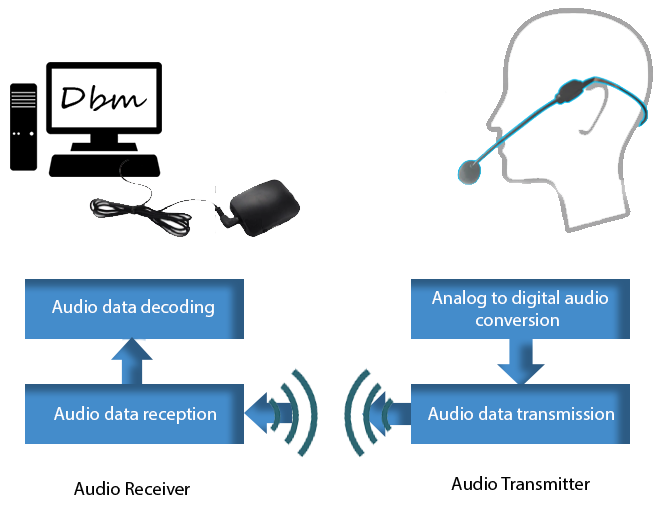
\includegraphics[width=13cm, height=12cm]{Audio Methodology}
  \caption{Audio Hardware General Methodology}
\end{figure}

\subsection{Controller Application}
Controller application plays several roles in the project. First of all, it is responsible for application of computer vision algorithms to detect marker and extract the position data. At least two camera perspectives are considered for position extraction. Manual calibration system aids in the setup and view port positioning of multiple cameras. Marker position data and audio data have to be synchronously written in the final output file.\\
Second, it is also responsible for decoding the orientation data. Orientation data is sent using encoded packet by Marker Hardware and received by the controller application. Orientation is extracted using quaternions. Euler angles then extracted using converted quaternion to avoid gimble lock. Position of the marker is extracted.\\
Third, it can play the lecture file before uploading the lecture. Lecture can be paused, resumed and replayed. also, the lecture can be annotated by the instructor i.e. topic and sub-topic markings. Audio and video quality can be controlled over performance of lecture play media.\\

\bigskip
\begin{figure}[h]
  \centering
  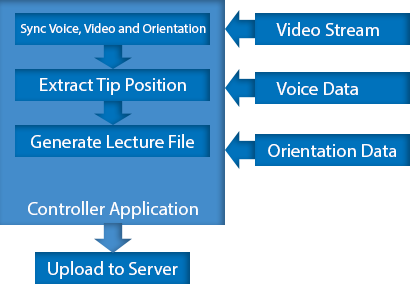
\includegraphics[width=13cm, height=11cm]{Controller Application Methodology}
  \caption{Controller Application General Methodology}
\end{figure}
\bigskip
\bigskip
\subsection{Player Application}
Just like media player, the player application plays the lecture. Common end user of Player Application is student. Player application has two version based on data availability.
\bigskip
\bigskip
\subsection{Offline Player}
Lecture file can be played on the computer via Offline Player with no interaction with internet at all. Typical end user is student. A student can rewind, play, pause, stop and resume while watching the lecture. As the lecture is being played by generated lecture file So, there is no compromise on quality.
\newpage
\begin{figure}[h]
  \centering
  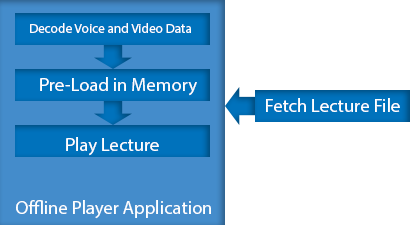
\includegraphics[width=13cm, height=8cm]{Player Application Methodology (Offline)}
  \caption{Offline Player Application General Methodology}
\end{figure}

\subsection{WebGL Player}
It is an online in-browser player that streams the lecture right in the webpage. Similar to video media player, flow of video can be controlled by user. This online player first loads its necessary packages and plugins before it could be fully functional. While browsing the lecture hierarchy, any lecture can be played by user and annotated by an instructor.

\begin{figure}[h]
  \centering
  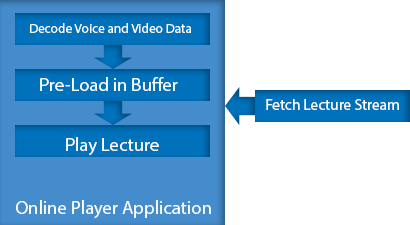
\includegraphics[width=13cm, height=8cm]{Player Application Methodology (Online)}
  \caption{Online Player Application General Methodology}
\end{figure}

\newpage
\subsection{Learning Management System}
LMS System that provides platform for playing online lectures, assignment submission and course content management. This module will act as a final deliverable when integrated with Online Lecture Player. This module consists of many sub-modules and functionalities. It also acts as an online portal for students and play important role in maintaining their profile. Below is further detailed discussion about this module. LMS developed for this project has other features including Administration, Access to high quality study material and learning data, email updates for students as well as teachers, fast delivery of learning material guided by the instructor and organized by existing institute, updates of emerging technologies to make students up-to-date and excel in their career in future. Report generation is another major advantage of the developed module. Using this functionality, instructor of the class can generate reports daily, weekly, monthly and so on. Also, reports are not only about the students. They can be about course material and Lecture data as well. Attendance of students and instructors as well can be maintained and reported easily. Concerned party can view the generated report at any time. Students can view timetable. Concerned instructor can suggest the adjustments to the timetable that administration can see and adjust accordingly. The application is web based so that accessibility of the system could be increased. Reliability and security are major concerns to the system. Administration can suspend the user by analysing the suspicious activity performed by the corresponding person.
\subsubsection{Entity Relationship Diagram}
\begin{figure}[h]
  \centering
  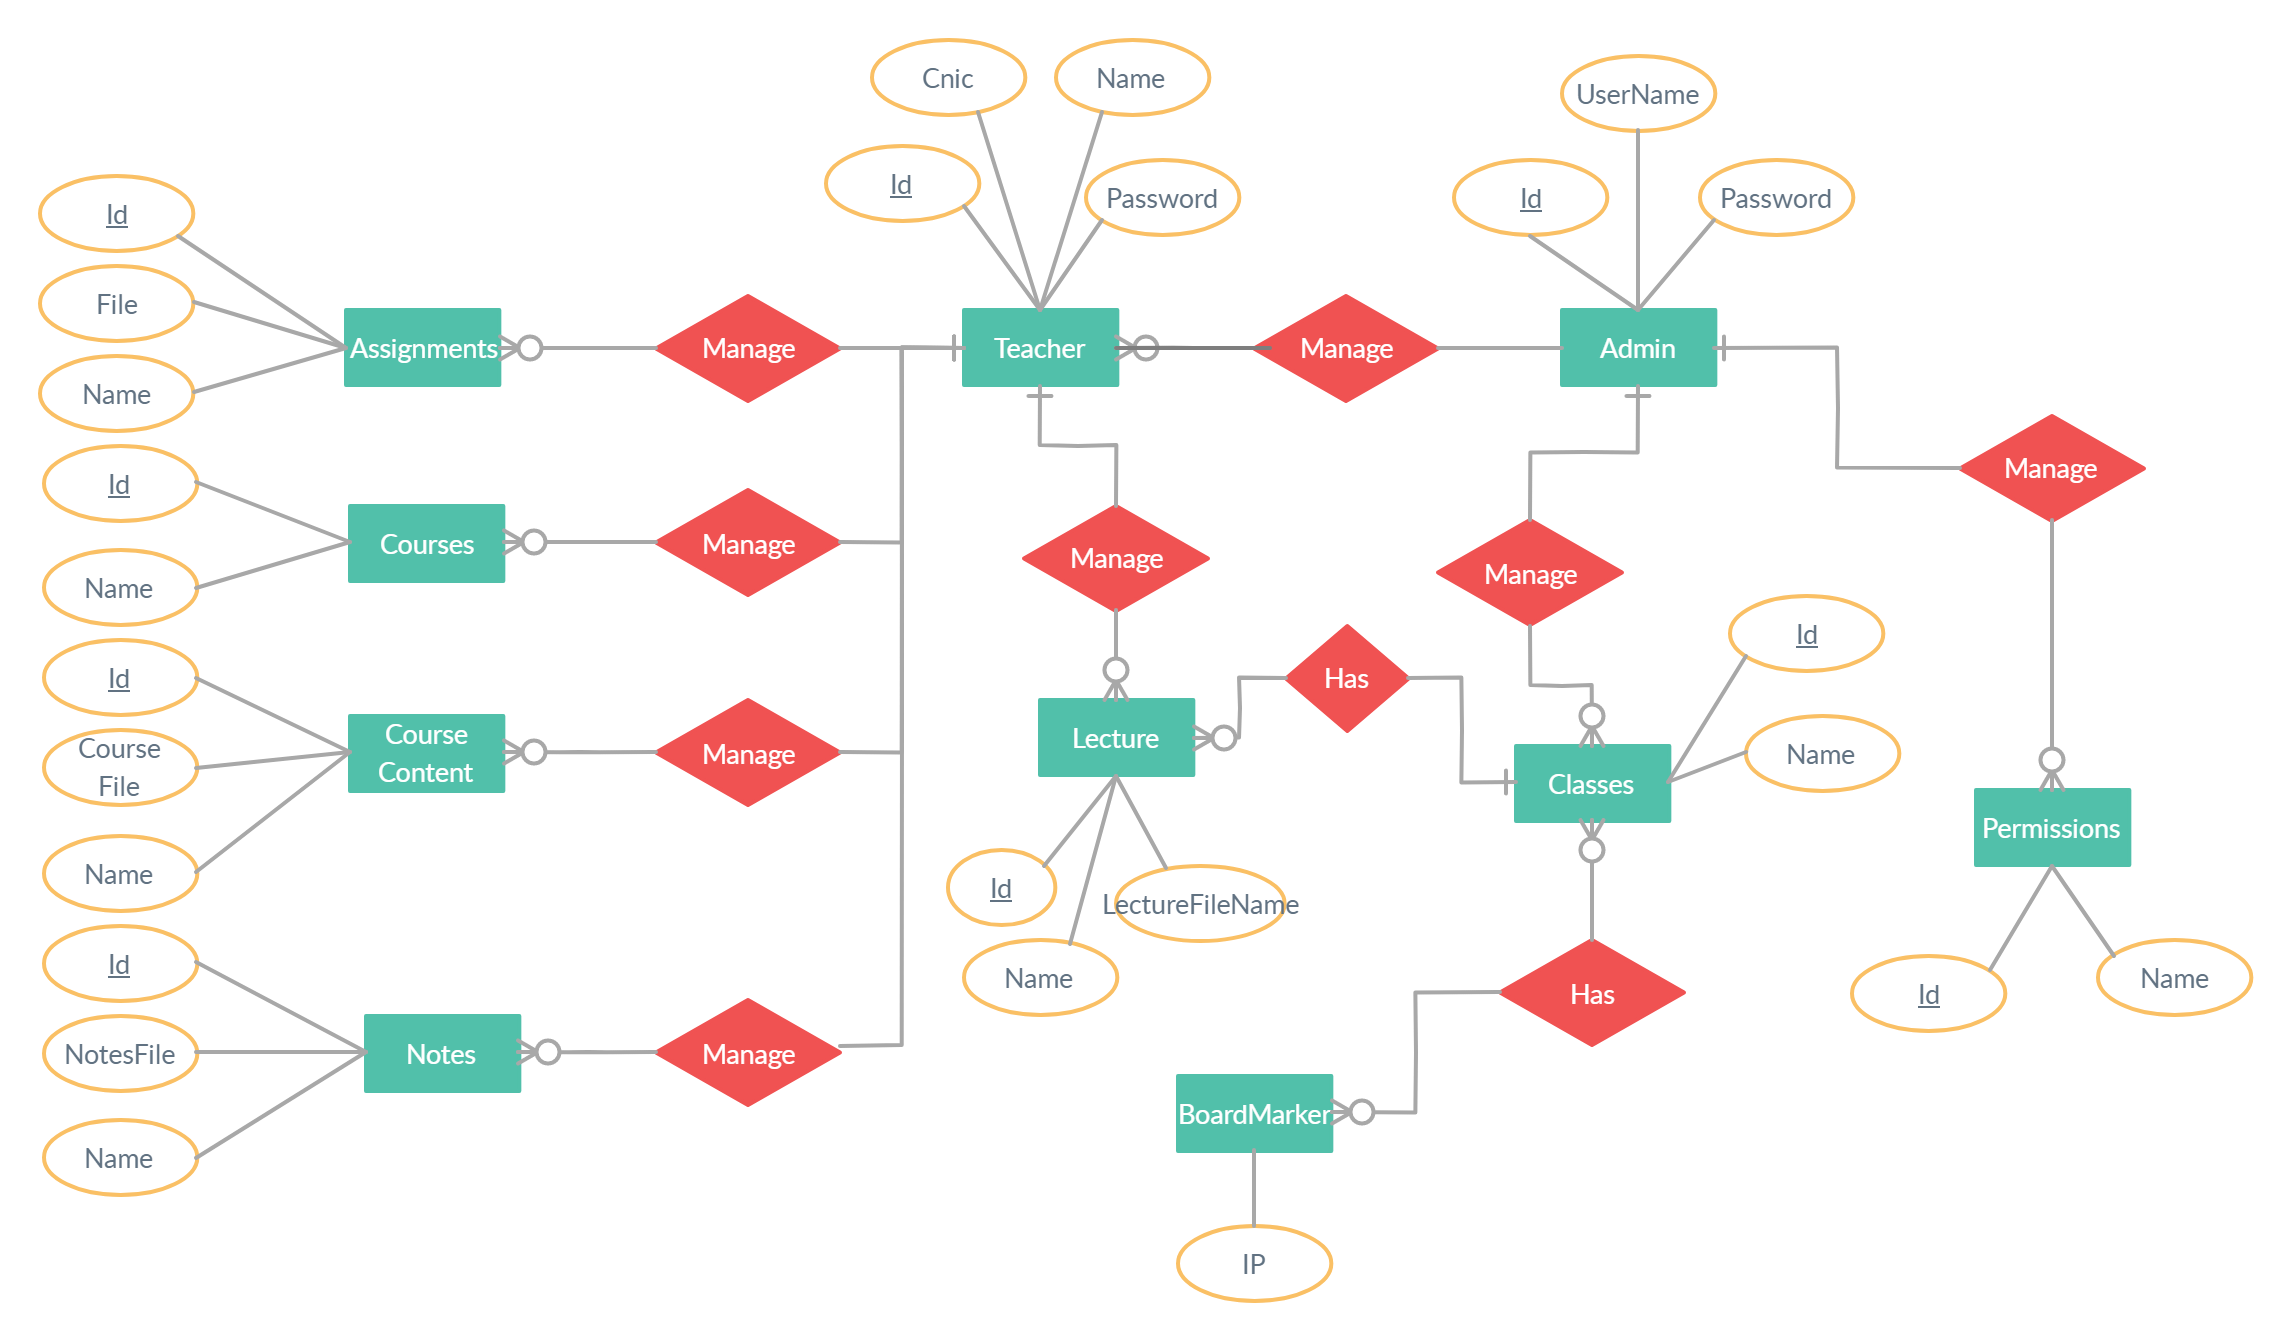
\includegraphics[width=13cm, height=7cm]{Entity Diagram}
  \caption{ER Diagram of LMS}
\end{figure}
\newpage


\subsubsection{Database Diagram}
\begin{figure}[h]
  \centering
  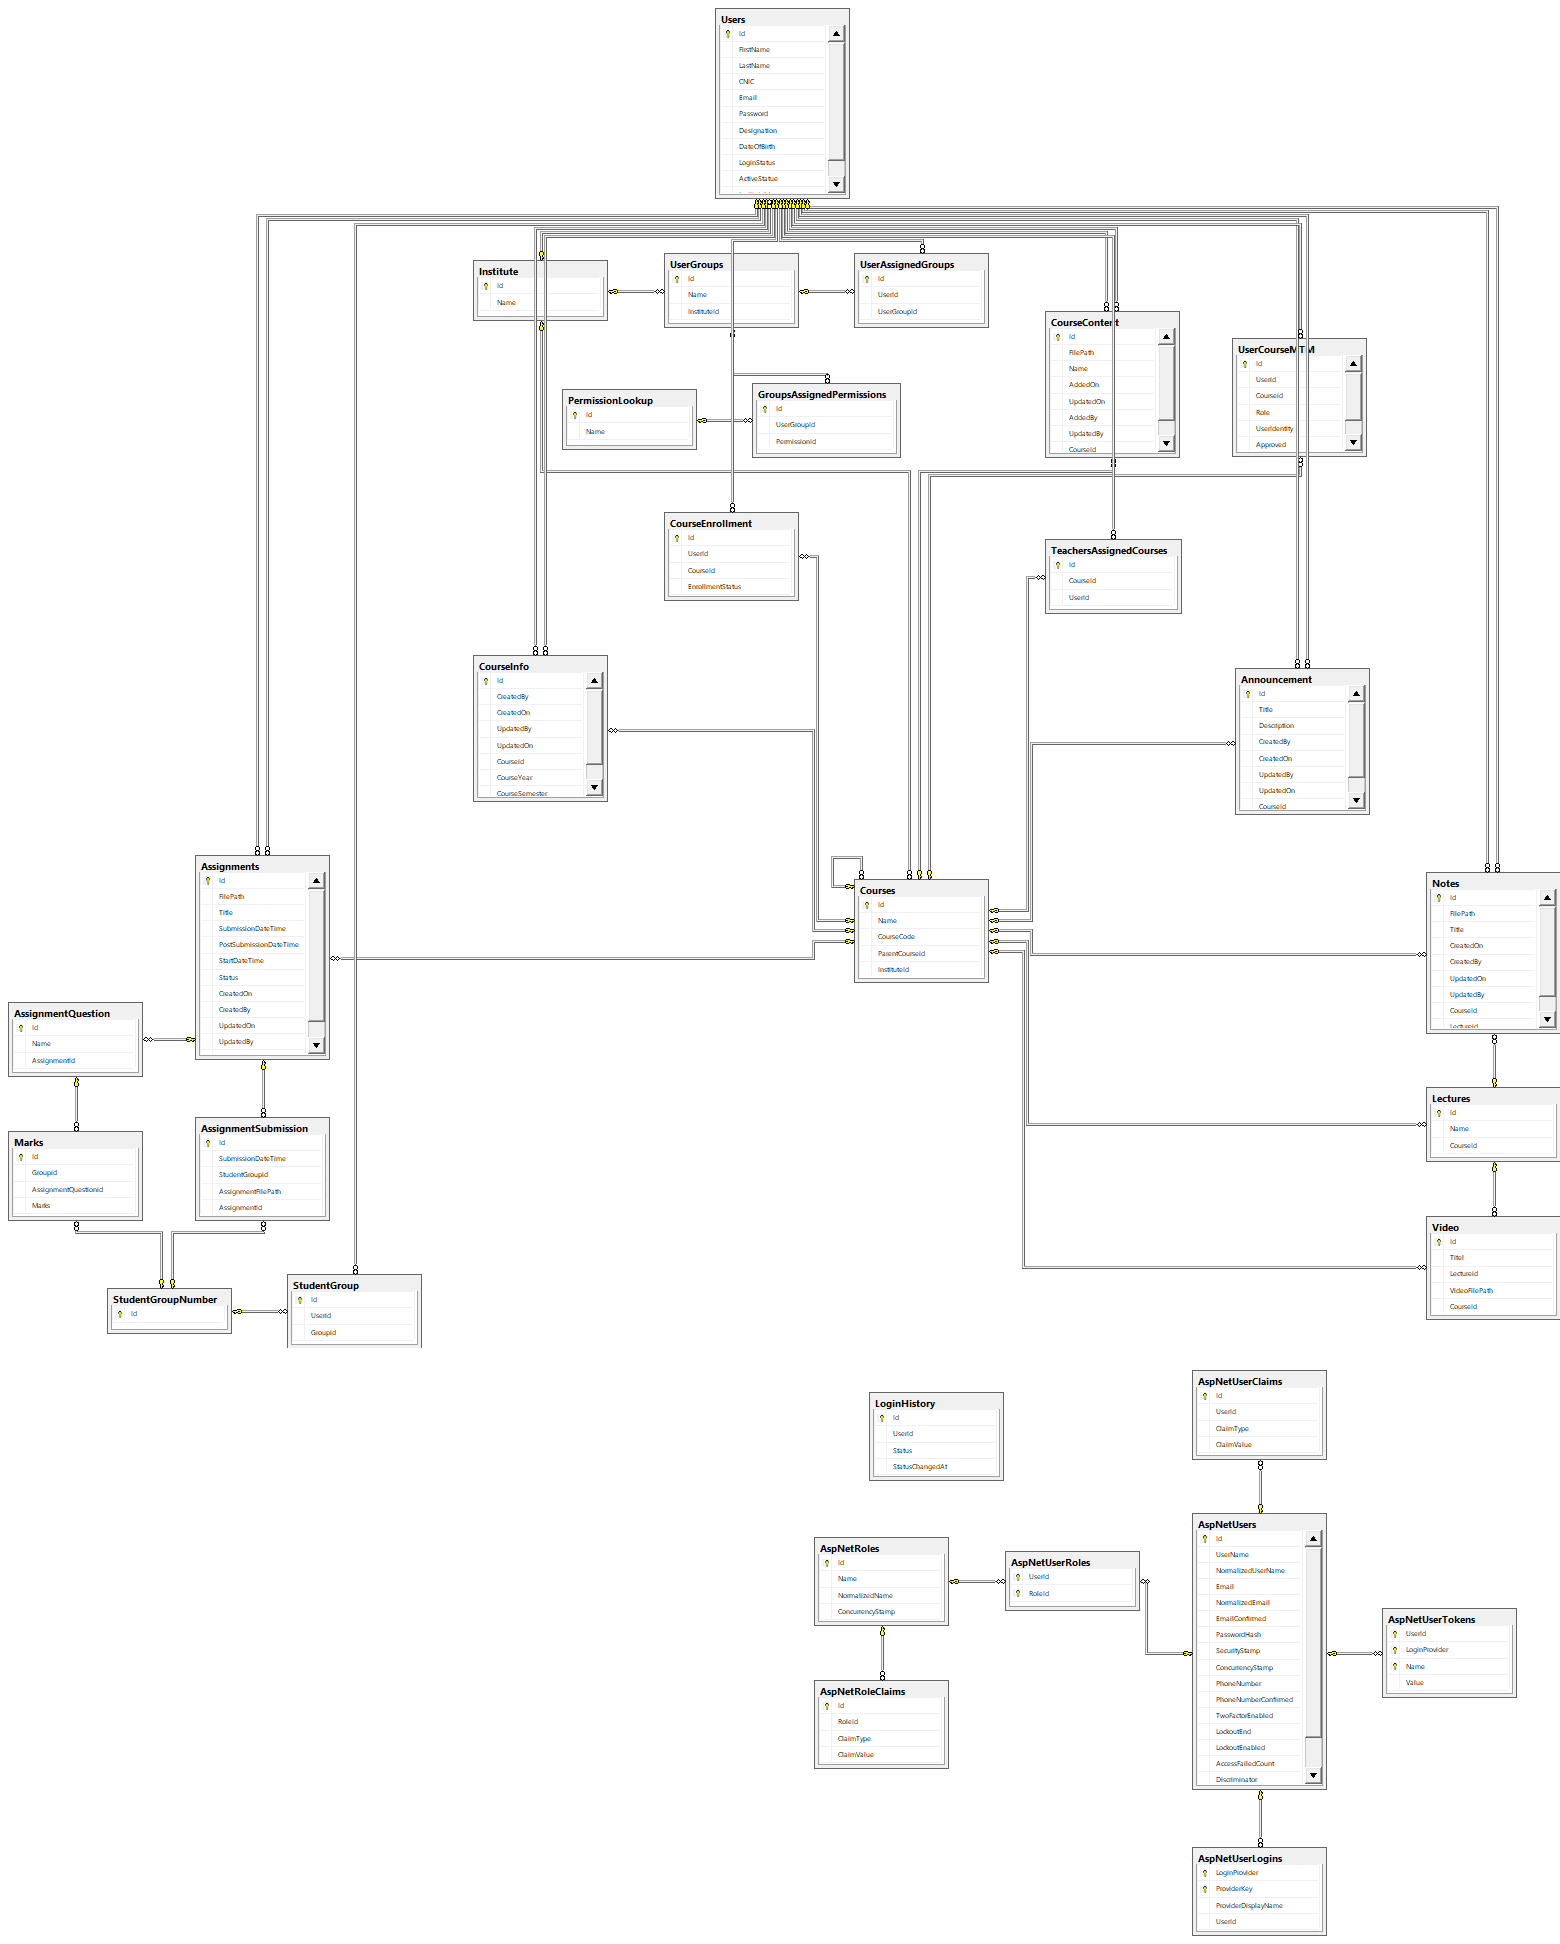
\includegraphics[width=15cm, height=13cm]{DBM_DB_Diagram}
  \caption{DB Diagram of LMS}
\end{figure}






%\begin{figure}[h]
%  \centering
%  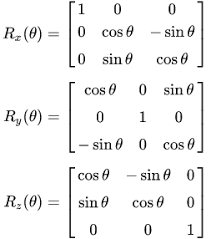
\includegraphics[width=1cm, height=1cm]{EulerAngles}
%%  \caption{General Flow of the Project}
%\end{figure}



















